% !TEX root = main.tex

\subsection{LCA of the Adaptive Solar Facade}

A breakdown of the embodied carbon emissions can be found in Figure  \ref{fig:embodied}. It can be seen that the largest emboodied global warming potential (GWP) contribution in the ASF comes from the solar panels, the electronics and the steel frame. 

\begin{figure}[H]
\begin{center}
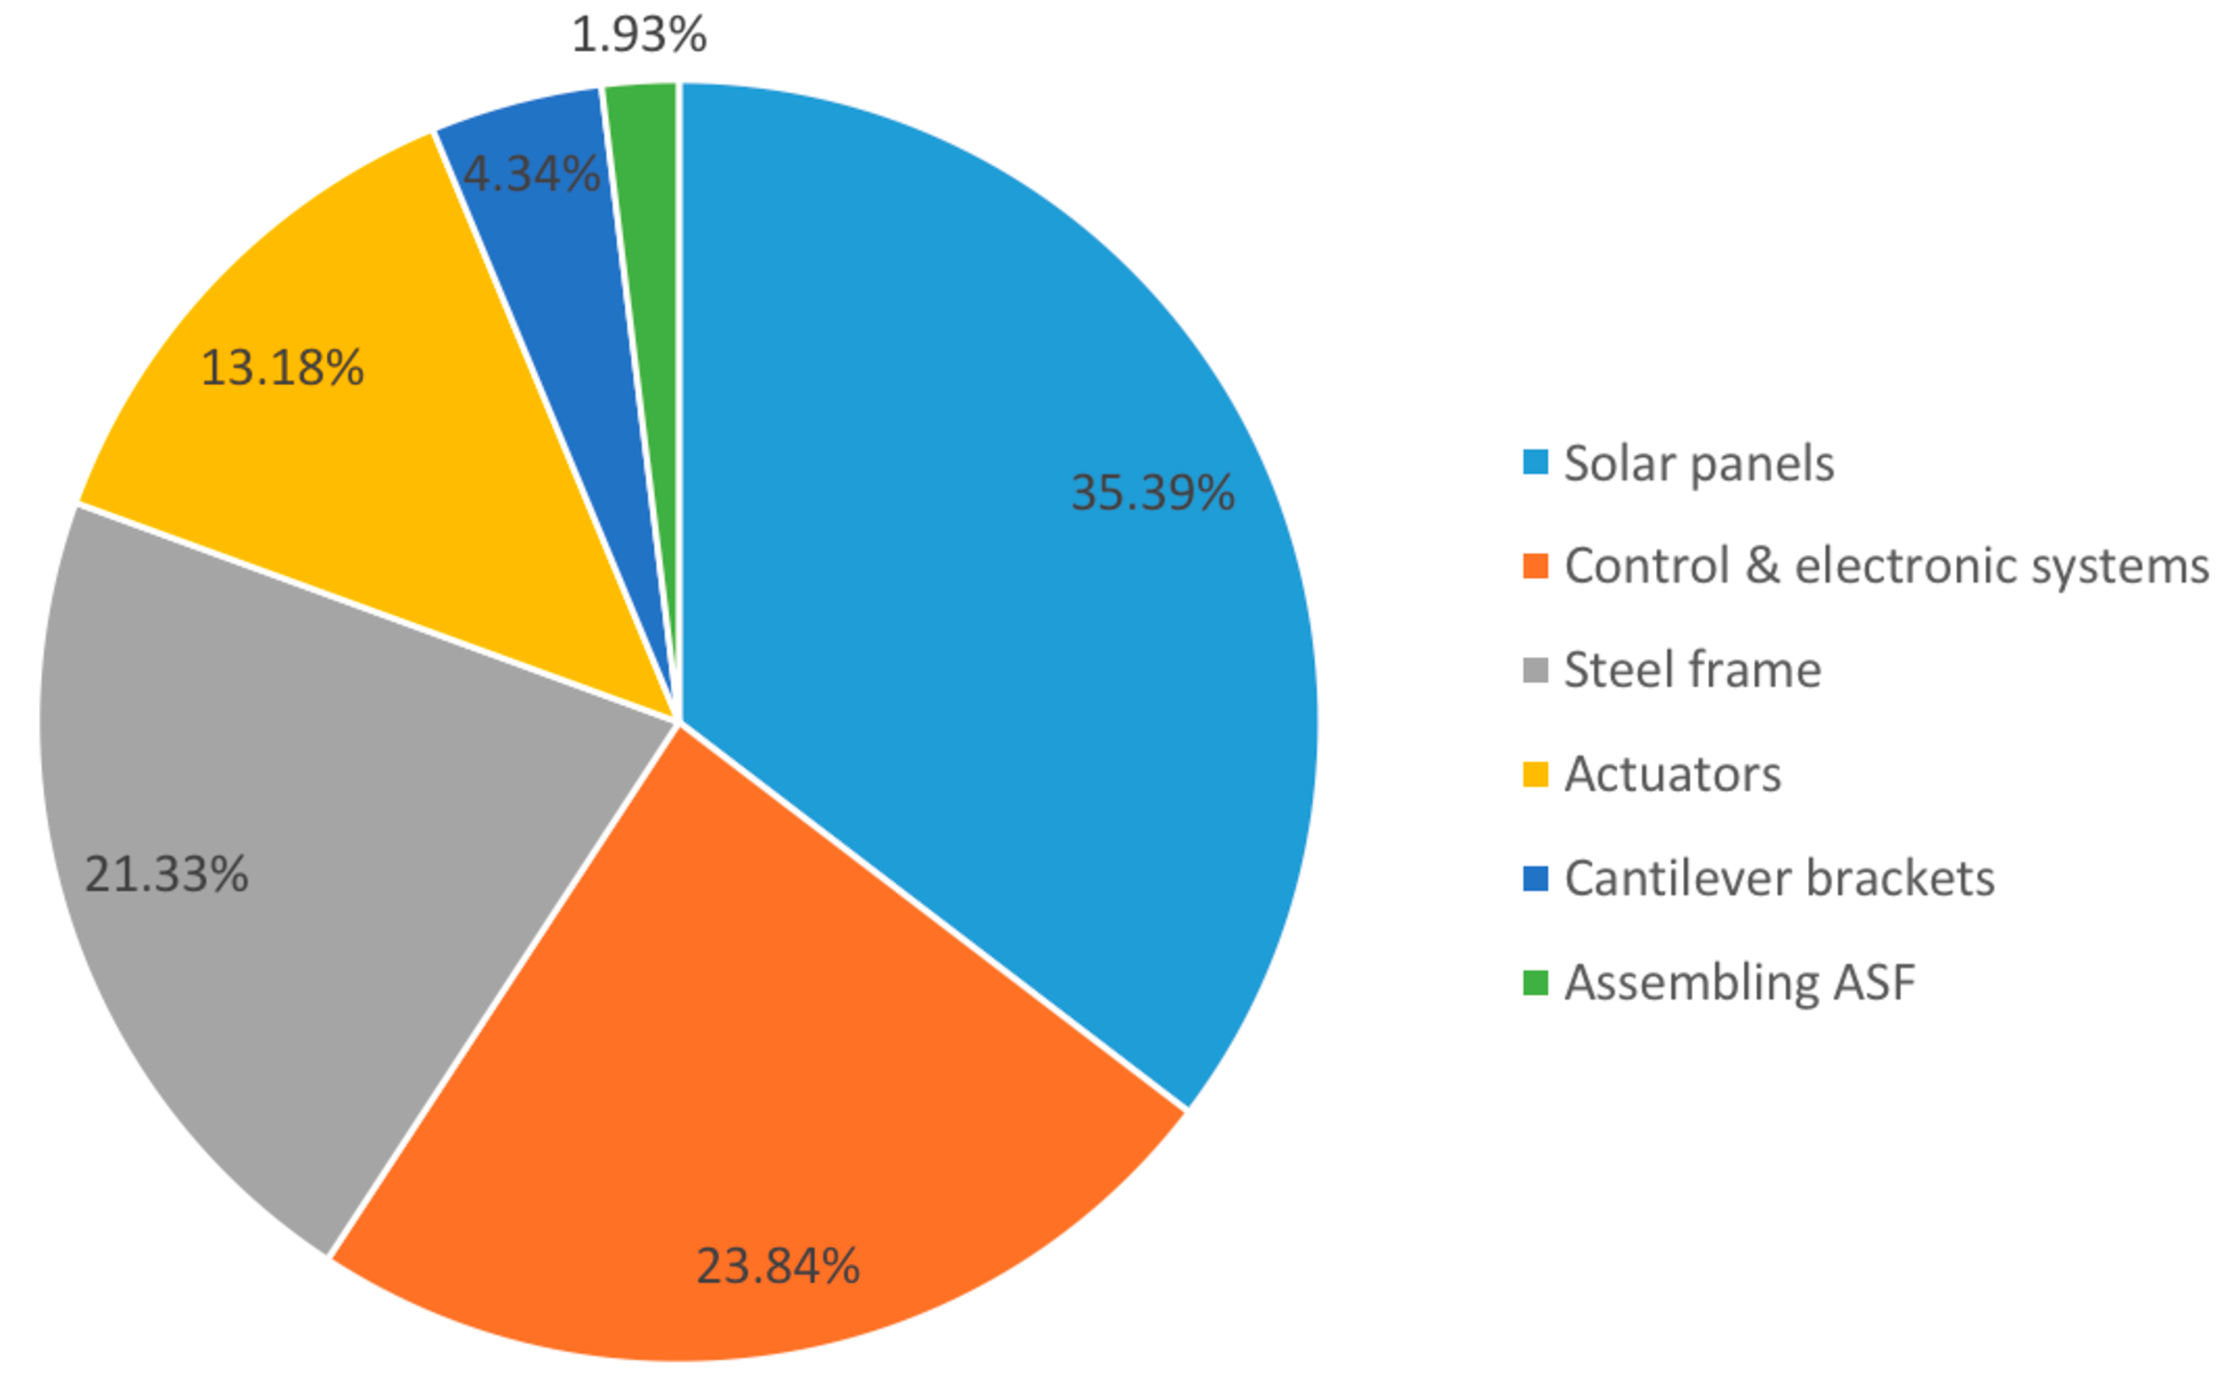
\includegraphics[width=10cm, trim= 0cm 0cm 0cm 0cm,clip]{pieembodied}
\caption{Breakdown of the embodied carbon emissions, it can be seen that xxxx has the greatest GWP contribution}
\label{fig:embodied}
\end{center}
\end{figure}


It is interesting to note that the choice of actuation system for an ASF can have a significant / minimal impact on the embodied emissions. [Elaborate further when results come in]

The operational energy consumption of the office space behind the ASF was compared to a case with a static louvered based shading system at 45$^\circ$ and a case with no shading at all. We calculated a total energy saving of 25\% compared to louvers at 45$^\circ$ and 56\% compared to a case with no facade shading \cite{jayathissa2015abs}. These results are sumarised in Figure \ref{fig:operational}. Note that this figure does not include on site electricity generation. 


\begin{figure}[H]
\begin{center}
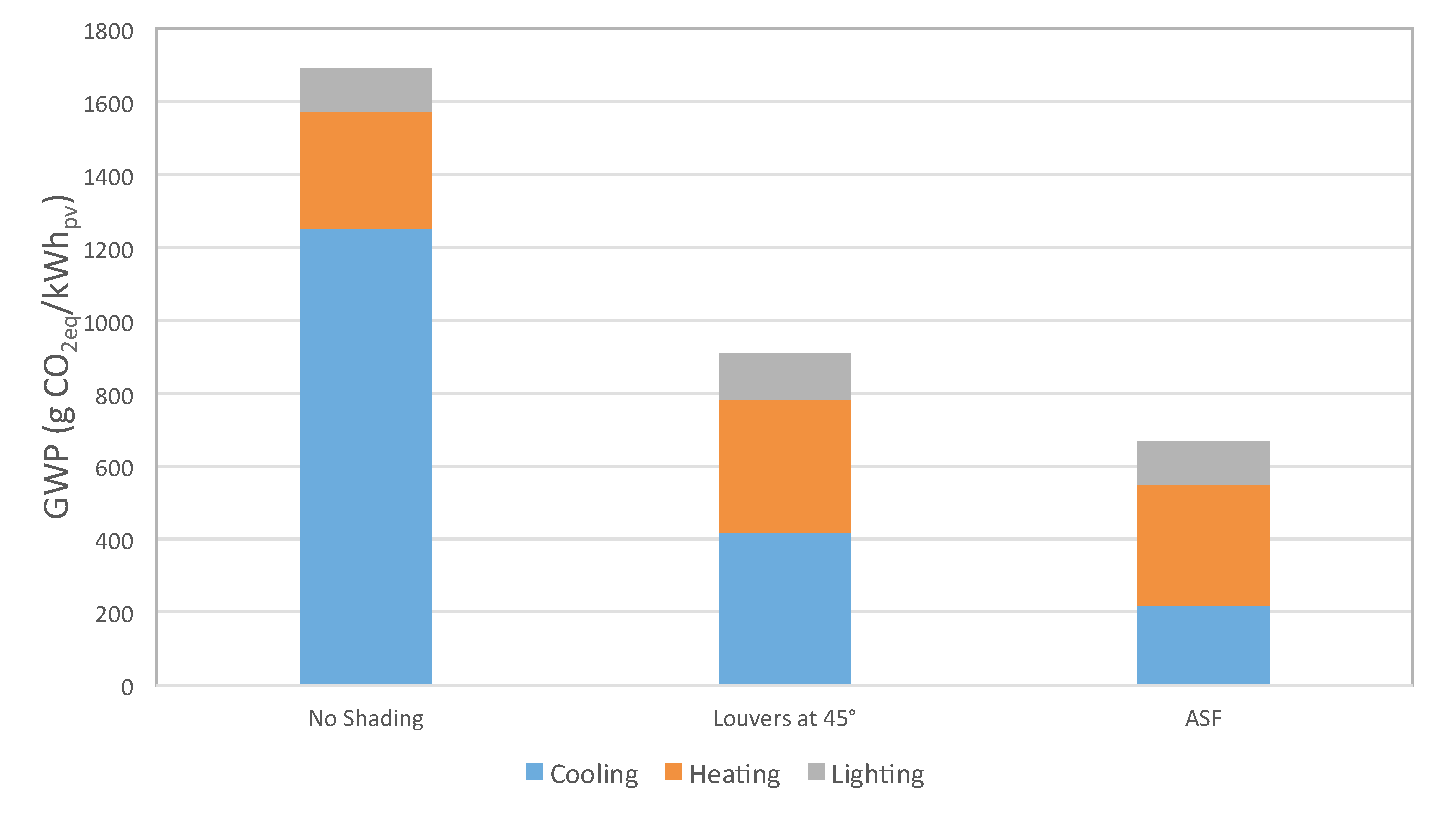
\includegraphics[width=10cm, trim= 0cm 0cm 0cm 0cm,clip]{buildingenergy.pdf}
\caption{Breakdown of the opperational carbon emissions, we can see a added savings of 24\% compared to a static louvered shading system and 56\% compared to no shading system at all}
\label{fig:operational}
\end{center}
\end{figure}

The total GWP of the ASF can be built up using a waterfall chart, Figure \ref{fig:waterfall}. To calculate the emission factor (gCO$_2$eq/kWh) we subtract the total embodied energy by the savings through our shading algorithm. We then add the GWP values for maintenance and disposal to achieve a total GWP over the 20 year life time of the ASF. This total is then used to calculate the emission factor of electricity produced by the ASF (126.8gCO$_2$/kWh).\\

It can be seen that the embodied GWP of the ASF is greater than a classical PV installation, however most of that initial investment is offset through the reduction of heating, cooling and lighting loads. Maintenance and disposal takes up roughly 10\% of all total carbon emissions.


\begin{figure}[H]
\begin{center}
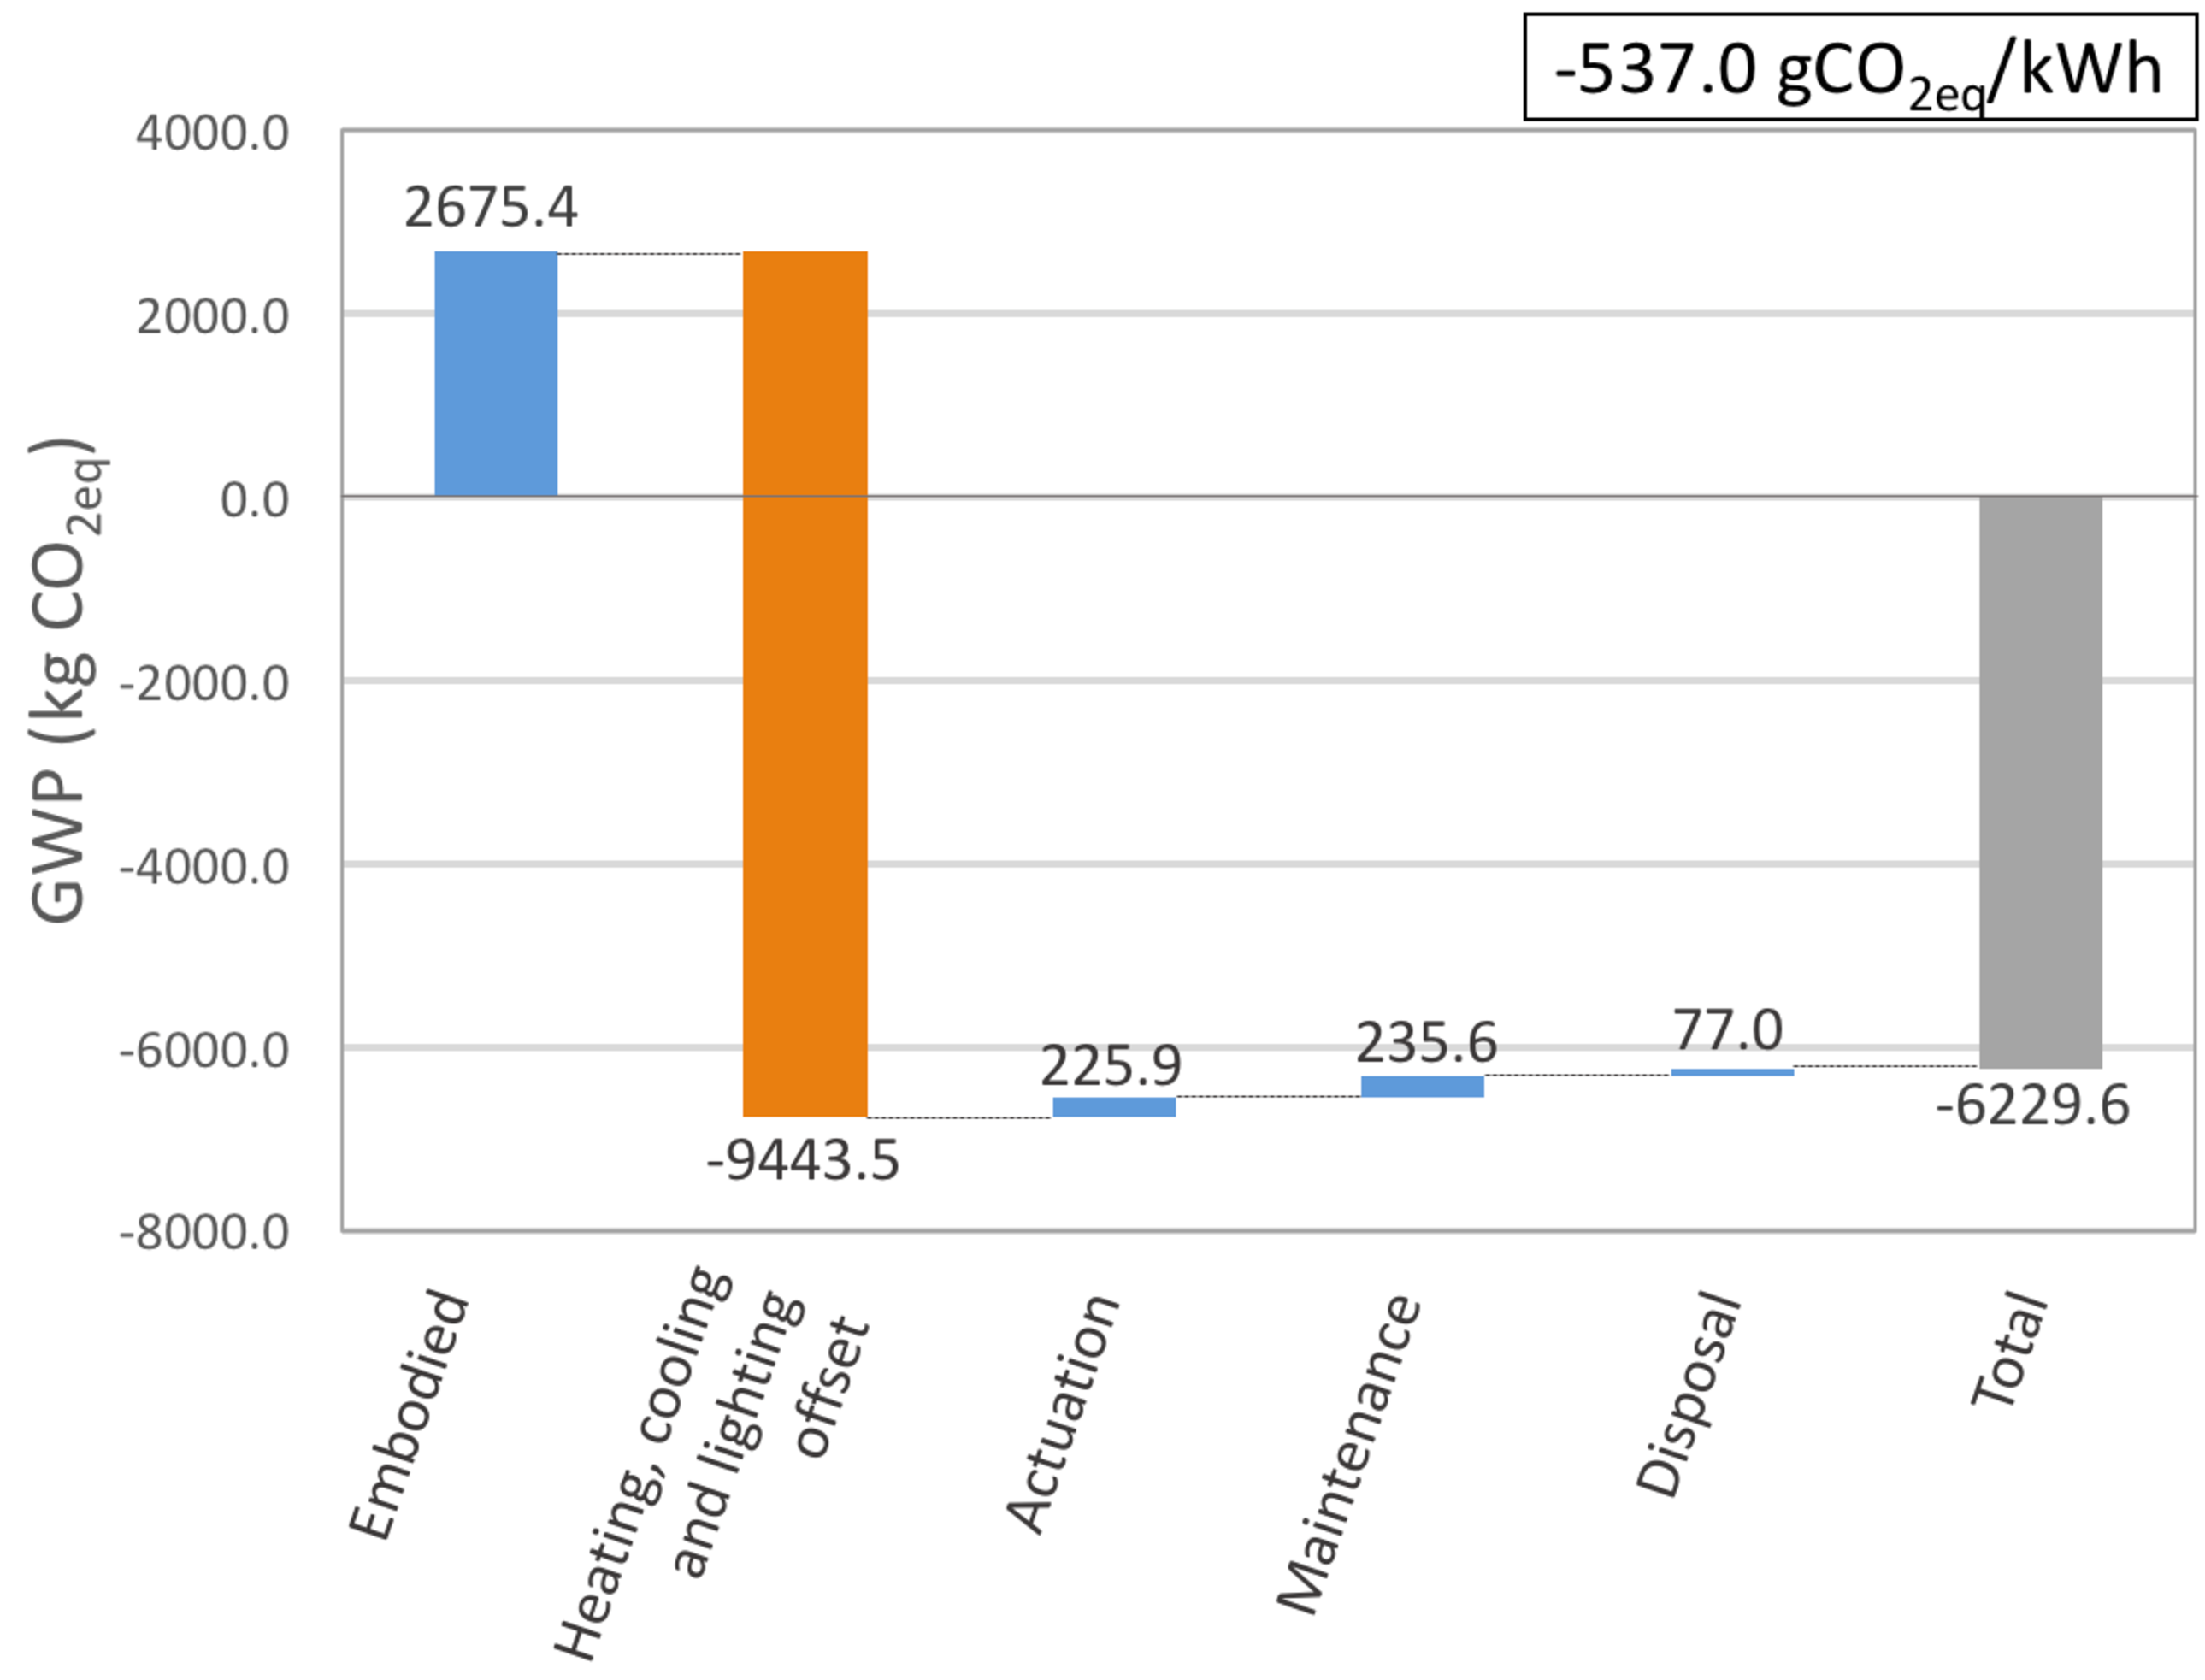
\includegraphics[width=10cm, trim= 0cm 0cm 0cm 0cm,clip]{waterfall}
\caption{Waterfall diagram of GWP of the ASF. The far left column details the embodied carbon emissions. The second bar details the emission reduction of the building through the smart shading algorithms of the ASF. The third column shows an increase of emissions through maintenance. The fourth column shows an increase in emissions in the disposal. This leaves us with a final emissions value. When we apply this value to Equation \ref{eq:solar} we obtain an emission factor per kwH of 126.8gCO$_2$/kWh.}
\label{fig:waterfall}
\end{center}
\end{figure}

\subsection{Global Distribution of GWP and Terrestrial Acidification}

The global distribution of embodied GWP emissions is focused in Europe, specifically Germany and Switzerland as most of the manufacturing is done in this region. It can be see however that emissions occur globally due the sourcing of primary materials from many locations around the world. Terrestrial acidification however is more interesting as it has a local impact compared to carbon emissions. It is interesting to note that China carries the greatest burden of terrestrial acidification from the ASF production. 
\begin{figure}[H]
\begin{center}
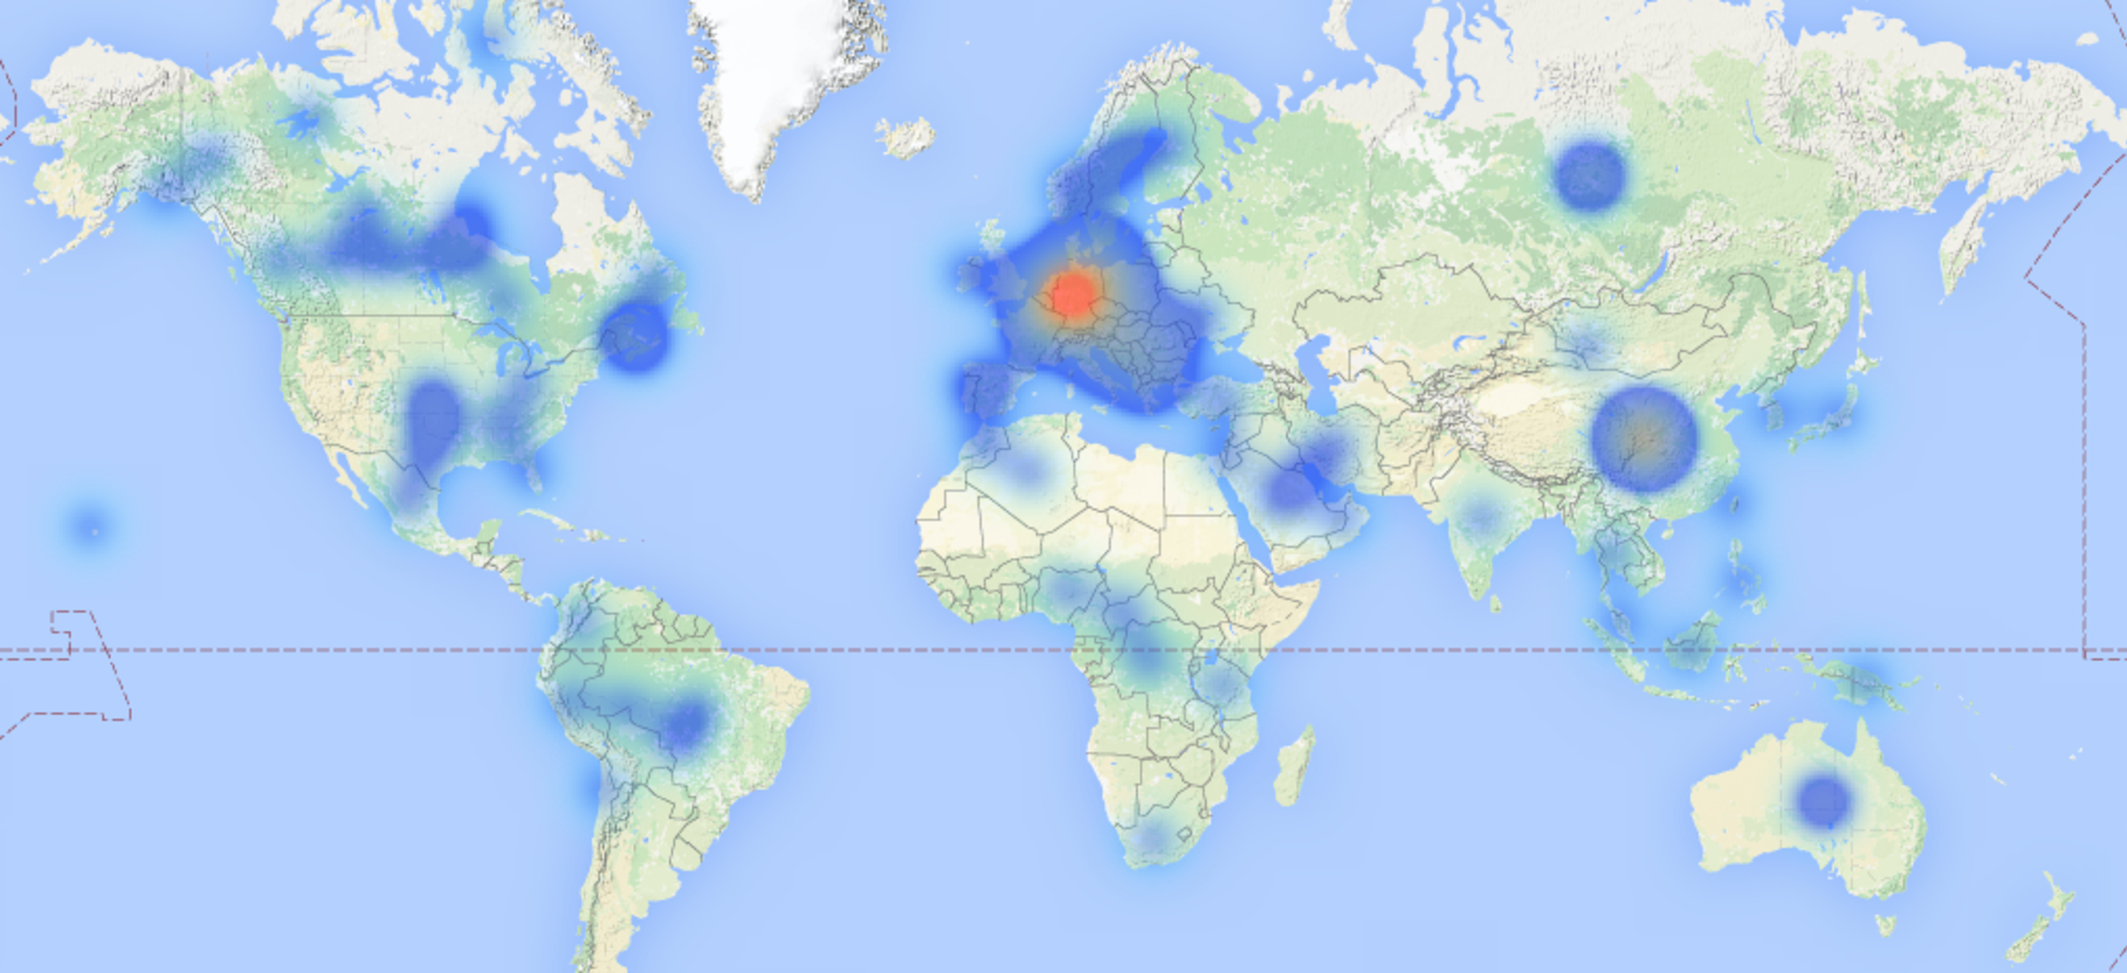
\includegraphics[width=10cm, trim= 0cm 0cm 0cm 0cm,clip]{mapGWP.pdf}
\caption{Global distribution of embodied GWP emissions}
\label{fig:mapGWP}
\end{center}
\end{figure}

\begin{figure}[H]
\begin{center}
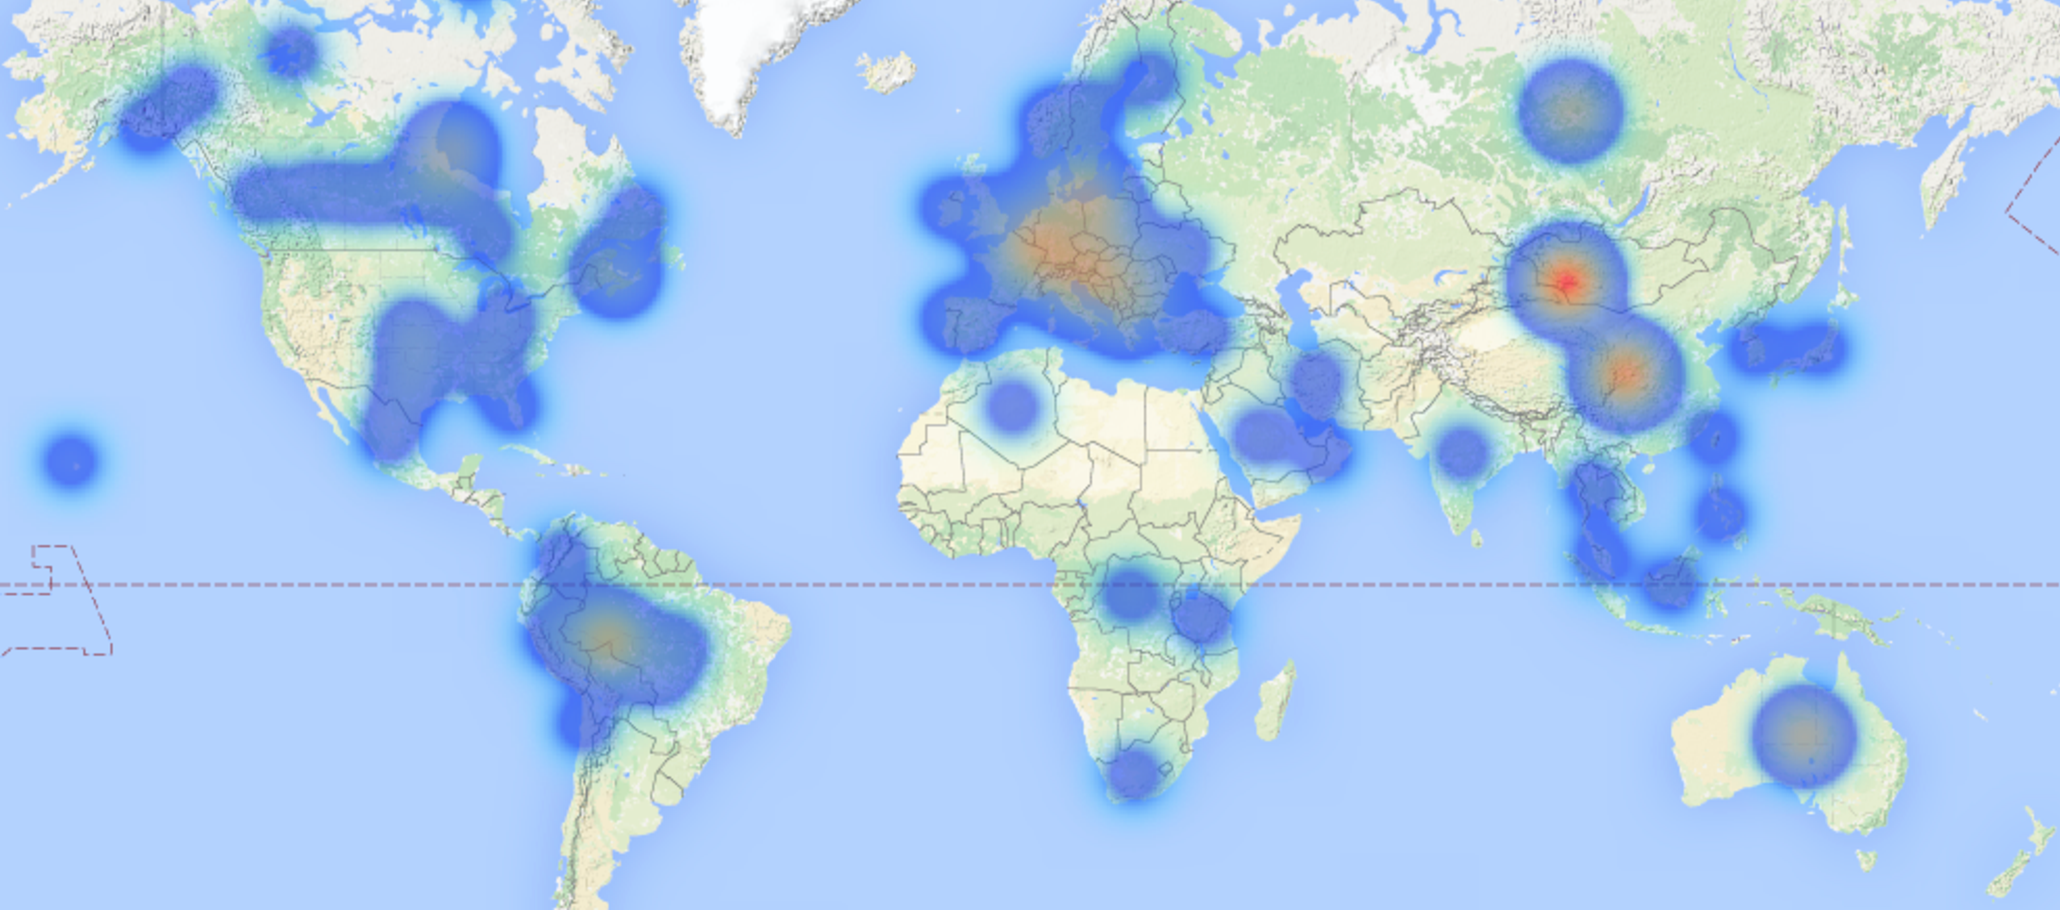
\includegraphics[width=10cm, trim= 0cm 0cm 0cm 0cm,clip]{mapacidification.pdf}
\caption{Global distribution of terrestrial acidification}
\label{fig:mapAcid}
\end{center}
\end{figure}



\subsection{Sensitivity Analysis}

Changing the assumptions can have a significant impact on the LCA result. Three assumptions were evaluated in the sensitivity analysis: Operation location, type of PV panels, and the type of actuation system. The inputs are summarised in Table \ref{tab:sens} with the results shown in Figure \ref{fig:sens}. \\

It can be seen that the operation location has a significant impact on the carbon saving potential. In Switzerland, we see a 6\% reduction compared to the average electricity mix. This is because the Swiss electricity mix is dominated by hydro and nuclear which has a very low GWP potential [citation needed]. In Germany on the other hand, the ASF has a 81\% reduction in carbon emissions as the emission factor of the electricity grid is roughly five times higher compared to Switzerland [citation needed]. The actuators and Pv panel type had a ...



\begin{table}
\centering
\begin{tabular}{lll}
\hline
Operation Location  & Switzerland & Germany \\
PV Panel type  & a-Si        & CIGS    \\
Actuator Type           & Servo Motor       & Soft Robotic Actuator   \\
\end{tabular}
\caption{Inputs to the Sensitivity Analysis Conducted}
\label{tab:sens}
\end{table}

\begin{figure}[H]
\begin{center}
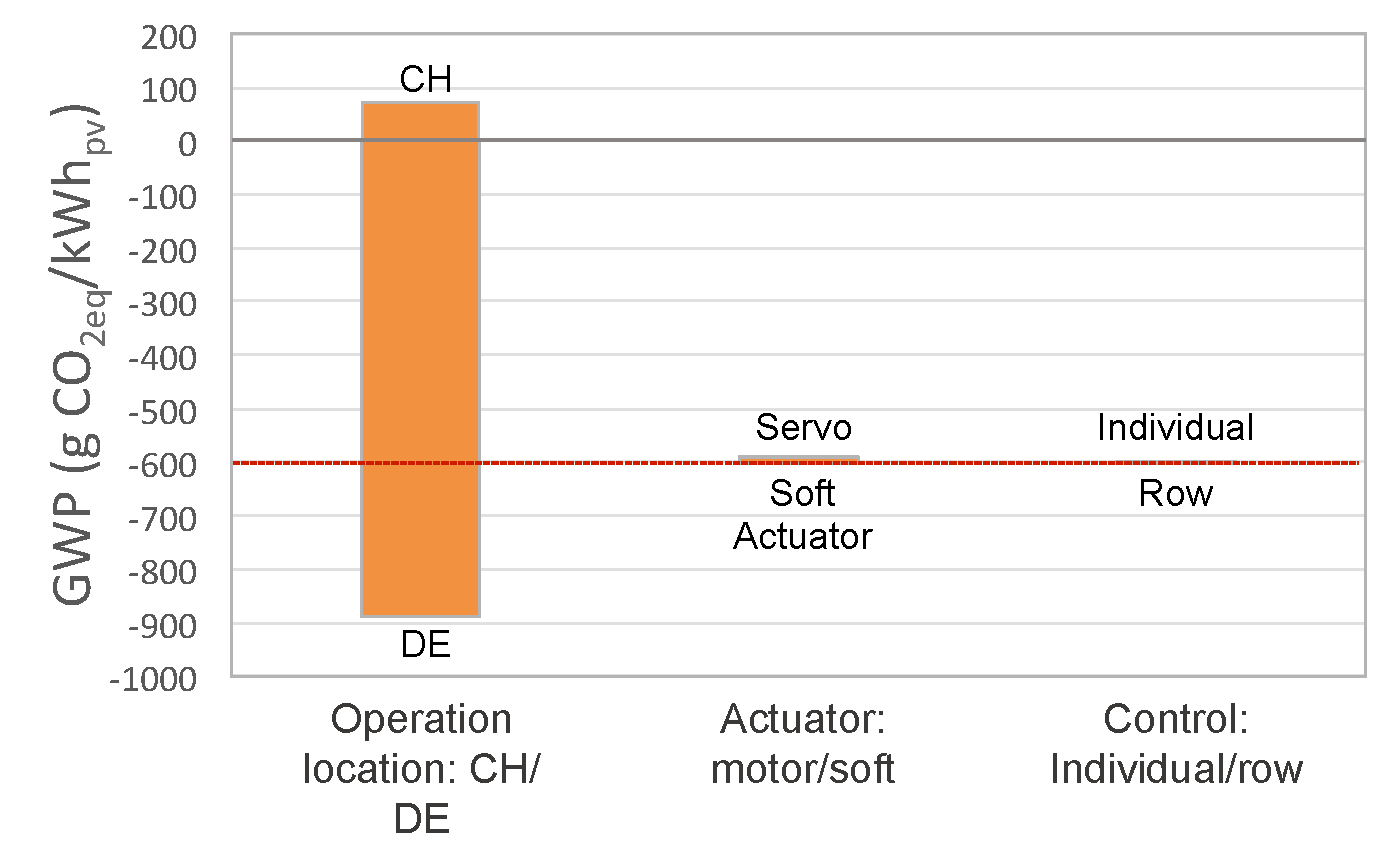
\includegraphics[width=10cm, trim= 0cm 0cm 0cm 0cm,clip]{sens.pdf}
\caption{Sensitivity analysis of the emission factor based on location of use, panel type, and actuator type (Under Heavy Construction)}
\label{fig:sens}
\end{center}
\end{figure}



% \begin{figure}[H]
% \begin{center}
% 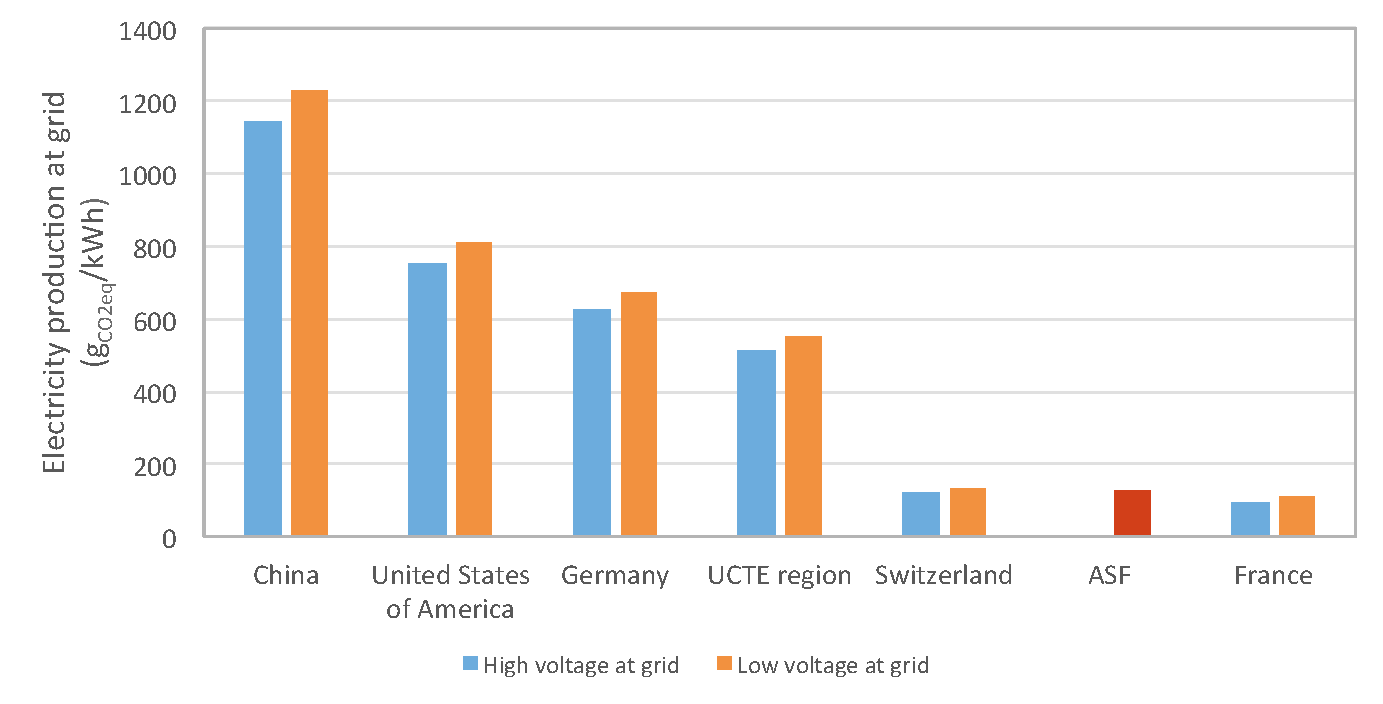
\includegraphics[width=10cm, trim= 0cm 0cm 0cm 0cm,clip]{regionGridMix.pdf}
% \caption{Comparison of the ASF when in operated in Switzerland when compared to other countries in the world that have similar climate conditions. Note that the data will have to change because we can't really compare (ASF in Switzerland) with Germany. We should be comparing the ASF in Germany with Germany}
% \label{fig:compReg}
% \end{center}
% \end{figure}



% - As input parameters of production processes are stochastic, a Monte Carlo simulation is used to include this stochastic behavior in the results, as shown in Figure \ref{fig:monte}...

% \begin{figure}[H]
% \begin{center}
% 
\includegraphics[width=10cm, trim= 0cm 0cm 0cm 0cm,clip]{monte}
% \caption{Monte carlo simulation based on input uncertainties}
% \label{fig:monte}
% \end{center}
% \end{figure}

% - Sourcing location greatly influences the embodied GWP. For photovoltaic panels, the majority of embodied emissions result from the use of electricity during production. The GWP per kwh of the Chinese electricity mix is 1145.8 ${\mathrm{gCO_2eq/kWh}}$, while in Switzerland this is only 119.6 ${\mathrm{gCO_2eq/kWh}}$.
% % cool - did we already discuss what other sensitivities to use?

% \begin{figure}[H]
% \begin{center}
% 
\includegraphics[width=10cm, trim= 0cm 0cm 0cm 0cm,clip]{sensitivity}
% \caption{Sensitivity analysis based on sourcing location}
% \label{fig:sensitivity}
% \end{center}
% \end{figure}
